\documentclass[]{article}
\usepackage[utf8]{inputenc}
\usepackage{amsmath}
\usepackage{amssymb}
\usepackage{graphicx}
\usepackage{geometry}
\usepackage{enumitem}
\usepackage{amsthm}
\usepackage{graphicx}
\usepackage{geometry}

\geometry{hmargin=2cm}

\title{Analyse}

\author{Arnaud Durand et Pierre Gervais}

% Environnement type théorème
\newtheorem{mythm}{Théorème}
\newtheorem{myproposition}{Proposition}
\newtheorem{myproperty}{Propriété}
\newtheorem{mylemma}{Lemme}

% Environnement type texte
\theoremstyle{remark}
\newtheorem{mynot}{Notation}
\newtheorem{myrem}{Remarque}
\newtheorem{myexer}{Exercice}
\newtheorem{myproof}{Preuve}
\newtheorem{myexmpl}{Exemple}

% Environnement de définition
\theoremstyle{definition}
\newtheorem{mydef}{Définition}

\setlist[itemize]{label=-}

% Carré de fin de preuve
\newcommand{\cqfd}{
	\hfill$\square$
}

% Définition de fonction
\newcommand{\func}[5]{
#1 ~ : ~ \left\{ \begin{array}{lcl}
	#2 & \longrightarrow & #3 \\
	#4 & \longmapsto & #5
\end{array}
\right.
}

\newcommand{\fun}[3]{
#1 ~ : ~ #2 \longrightarrow #3
}

\begin{document}

\maketitle

\tableofcontents

\part{Calcul propositionnel}

\section{Syntaxe}

Le \textit{calcul propositionnel} est un langage \textit{inductivement} et \textit{librement engendré} par un ensemble de règles.

C'est à dire qu'une formule ne peut pas être obtenu de deux façons différentes.

\begin{mydef}	
	Soit $\mathcal{P}$ un ensemble de constantes propositionnelles, on définit $\mathcal{F}_\mathcal{P}$ le calcul propositionnel sur $\mathcal{P}$ obtenu par les règles suivantes :
	\begin{itemize}
		\item si $p \in \mathcal{P}$, alors $p \in \mathcal{F}_\mathcal{P}$
		
		\item $\perp \in \mathcal{F}_\mathcal{P}$
		
		\item si $F \in \mathcal{F}_\mathcal{P}$, alors $\left(\neg F\right) \in \mathcal{F}_\mathcal{P}$
		
		\item si $F, G \in \mathcal{F}_\mathcal{P}$ alors $(F \lor G), (F \land G), (F \rightarrow G) \in \mathcal{F}_\mathcal{P}$
	\end{itemize}
\end{mydef}

\begin{mynot}
	S'il n'y a pas d'ambiguïté, on notera $\mathcal{F}_\mathcal{P} = \mathcal{F}$
\end{mynot}

\begin{mydef}
	Une définition alternative de $\mathcal{F}$ est $\displaystyle \mathcal{F} = \bigcup_{n \geqslant 0} \mathcal{F}_n$
	où
	\begin{itemize}
		\item $\mathcal{F}_0 = \mathcal{P}$
		\item $\mathcal{F}_{n+1} = \mathcal{F}_n \cup \{(\neg F) ~ | ~ F \in \mathcal{F}_n)\} \cup \{(F \star G) ~ | ~ F, G \in \mathcal{F}_n, ~ \star \in \{\land, \lor, \rightarrow\}\}$, avec $n \geqslant 0$
	\end{itemize}
	
	On définit la \textit{hauteur} d'une formule $F$ par le plus petit $n$ tel que $F \in \mathcal{F}_n$.
\end{mydef}

\begin{myrem}
	Ce langage est fortement parenthésé et toute formule peut être représentée par un arbre de décomposition.
\end{myrem}

\begin{figure}[h!]
	\centering
	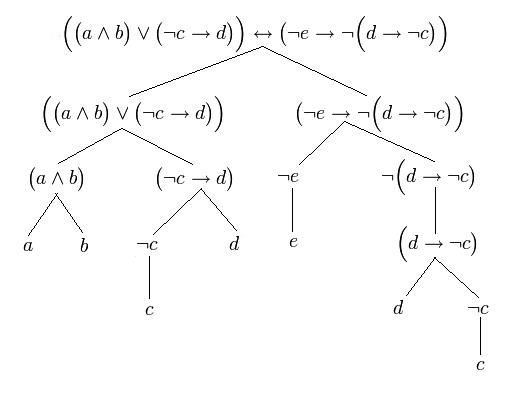
\includegraphics{Arbre_decomposition}
	\caption{Arbre de décomposition}
\end{figure}

\begin{myproperty}{Propriété de lecture unique}

	Pour tout $F \in \mathcal{F}$, un seul de ces cas est vrai :
	
	\begin{enumerate}
		\item $F \in \mathcal{P}$
		\item Il existe un \textit{unique} $G \in \mathcal{F}$ tel que $F = (\neg G)$

		\item Il existe d'\textit{uniques} $G,H \in \mathcal{F}$ et $\star \in \{\lor, \land, \rightarrow \}$ tels que $F = G \star H$
	\end{enumerate}

	C'est-à-dire que toute formule ne peut se décomposer que d'une seule façon.
\end{myproperty}

\subsection{Raisonnements}

On démontrera généralement les propriétés s'appliquant à $\mathcal{F}$ par induction :
pour démontrer une proposition $A$ s'appliquant à $\mathcal{F}$, on la démontre sur $\mathcal{P}$ et pour tout $(F \star G)$ et $(\neg F)$ où on suppose que $F, G \in \mathcal{F}$ vérifient $A$ et $\star \in \{\land, \lor, \rightarrow\}.$

\subsection{Définition alternative de $\mathcal{F}_\mathcal{P}$}

Soit $\Sigma = \mathcal{P} \cup \{(, ), \neg, \land, \lor, \rightarrow, \perp \}$, $\Sigma^*$ est l'ensemble des mots sur $\Sigma$.

\begin{myexmpl}
	\leavevmode
	\begin{itemize}
		\item $F = (\land \neg x_1)(( \in \Sigma^*$
		\item $F = (\neg x_1) \in \Sigma^*$
	\end{itemize}
\end{myexmpl}

\begin{mydef}
	$\mathcal{F}$ est le plus petit sous-ensemble de $\Sigma^*$ contenant $\mathcal{P} \cup \{\perp\}$ et \textbf{clos} par les opérations
	\begin{enumerate}
		\item $(F, G) \longmapsto (F \lor G)$
		\item $(F, G) \longmapsto (F \land G)$
		\item $(F, G) \longmapsto (F \rightarrow G)$
	\end{enumerate}
\end{mydef}

\begin{myrem}
	On peut montrer que les deux définitions correspondent.
	$\mathcal{F}$ satisfait la propriété de lecture unique (voir TD). 
\end{myrem}

\subsubsection{Sous-formule, hauteur, arbre de décomposition}

\begin{mydef}
	Soit $F \in \mathcal{F}$, on définit $\mathcal{S}(F)$ l'ensemble des \textit{sous-formules de $F$} telles que
	
	\begin{itemize}
		\item si $F \in \mathcal{P}$, $\mathcal{S}(F) = \{F\}$
		\item si $F = (\neg G)$ alors $\mathcal{S}(F) = \{F \} \cup \mathcal{S}(G)$
		\item si $F = (G \star H)$ où $\star \in \{\land, \lor, \rightarrow \}$, alors $\mathcal{S}(F) = \{F\} \cup \mathcal{S}(G) \cup \mathcal{S}(H)$
	\end{itemize}
\end{mydef}

TODO : vérifier dernier point

\begin{mydef}
	Soit $F \in \mathcal{F}$ on définit la \textit{hauteur} $h(F)$ de $F$ par
	\begin{itemize}
		\item $h(F) = 0$, si $F \in \mathcal{P}$
		\item si $=(\neg G)$, alors $h(F) = 1 + h(G)$
		\item si $F = (G \star H)$, alors $h(F) = 1 + \max\{h(G), h(H)\}$
	\end{itemize}
\end{mydef}

\begin{mydef}
	Soit $F \in \mathcal{F}$, l'\textit{arbre de décomposition de $F$} $arb(F)$ est un graphe étiqueté défini par
	
	\begin{enumerate}
		\item si $F \in \mathcal{P}$, $arb(F)$ est réduit à un sommet étiqueté par $F$.
		\item si $F = (\neg G)$, alors $arb(F) = \neg - arb(G)$
		\item si $F = (G \star H)$, alors $arb(F) = G - \star - H$
	\end{enumerate}
\end{mydef}

\begin{mynot}
	Soit $F$ une formule, $var(F)$ est l'ensemble des variables de $F$, $occ(F)$ est le multi-ensemble des variables de $F$ et $arb(F)$ est le graphe
	\begin{itemize}
		\item dont les sommets sont $V$
		\item et muni d'une fonction d'étiquetage $\lambda ~ : ~ V \longrightarrow \{\neg, \perp, \lor, \land, \rightarrow \} \cup var(F)$.
	\end{itemize}
\end{mynot}

\begin{myrem}
	Toutes les définitions sont univoques par la propriété de lecture unique.
\end{myrem}

\begin{myrem}
	On définit la hauteur d'une formule par la hauteur de son arbre de décomposition, c'est-à-dire la distance maximum entre les feuilles et la racine. 
\end{myrem}

\begin{mynot}
	\leavevmode
	\begin{itemize}
		\item $\top$ comme abréviation pour $(\perp \rightarrow \perp)$
		\item $(p \longleftrightarrow q)$ pour $(p \leftarrow q) \land (p \rightarrow q)$
		\item $\bigwedge\limits_{i=1}^n A_i = (((A_1 \land A_2) \land A_3)... \land A_n)$
	\end{itemize}
\end{mynot}

\section{Sémantique}

On s'intéresse à des propositions dont la valeur de vérité est soit vrai soit faux. On a besoin d'une \textbf{interprétation} (en terme de vrai ou faux) de ces constantes propositionnelles.

\begin{mydef}
	Une \textit{valuation} est une fonction $v ~ : ~ \mathcal{P} \longrightarrow \{0, 1\}$.
	Étant donné une valuation $v$, on définit l'\textit{interprétation} $\fun{\overline{v}}{\mathcal{F}}{\{0, 1\}}$ comme ceci
	\begin{itemize}
		\item si $F = p \in \mathcal{P}$ alors $\overline{v}=v(p)$
		\item si $F = (\neg G) \in \mathcal{P}$ alors $\overline{v}(F) = 1$ si et seulement si $\overline{v}(G) = 0$
		\item $\overline{v}(\perp)=0$
		\item $\overline{v}(F \land G) = 1$ si et seulement si $\overline{v} (F) = \overline{v} (G) = 1$
	\end{itemize}
\end{mydef}

On peut décrire l'interprétation d'une formule par sa \textit{table de vérité} :

$$
	\begin{array}{|c|c||c|c|c|}
		\hline
		F & G & \neg G & F \land G & F \rightarrow G \\
		\hline
		0 & 0 & 1 & 0 & 1 \\
		\hline
		0 & 1 & 1 & 0 & 1 \\
		\hline
	\end{array}
$$

On définit formellement la \textit{table de vérité} par une fonction $\fun{v}{\{0, 1\}^\mathcal{P}}{\{0, 1\}}$

\begin{mydef}
	\leavevmode
	\begin{itemize}
		\item $F \in \mathcal{F}$ est dit \textit{satisfaisable} s'il existe une valuation $v$ de $\mathcal{P}$ tel que $\overline{v}(F)=1$
		\item $F$ est dit \textit{valide} si pour toute valuation $v$ de $\mathcal{P}$, $\overline{v}(F) = 1$, on dit aussi que $F$ est une \textit{tautologie}.
		\item $F$ et $G$ sont dites \textit{équivalentes}, notées $F \equiv G$, si pour toute valuation $v$, $\overline{v}(F)=\overline{v}(G)$
	\end{itemize}
\end{mydef}

\begin{myexer}
	Vérifier que $F \equiv G$ si et seulement si $F \leftrightarrow G$ est valide.
\end{myexer}

\begin{myproposition}
	Pour tout $F \in \mathcal{F}$, $F$ est satisfaisable si et seulement si $(\neg F)$ n'est pas valide.
\end{myproposition}

\section{Exemples de formalisation}

\subsection{Contraites de compatibilité/exclusion}

\paragraph{Problème :}On possède $n$ produits chimiques à ranger dans $k \leqslant n$ conteneurs. Certains produits ne peuvent pas être stockés ensemble dans un conteneur.

La contrainte est donnée sous la forme d'un ensemble $\mathcal{L} \subseteq [n]$ tel que $I = \{i_1, ..., i_k\} \subseteq \mathcal{L}$ si et seulement si les produits $i_1, .., i_k$ ne peuvent pas être stockés ensemble.

\paragraph{Enjeu :}
Écrire une formule propositionnelle $F$ telle que $F$ est satisfaisable si le problème a une solution.

Les variables propositionnelles $\mathcal{P}=p(i, j), ~ i \leqslant n, ~ j \leqslant k$ sont interprétées par "le produit chimique $i$ est dans le camion $j$".

On exprime deux propositions :
\begin{itemize}
	\item Chaque produit se trouve dans un unique conteneur :
	$F = \underbrace{\left(\bigwedge\limits_{i \leqslant n} \left(\bigvee\limits_{j \leqslant k} p(i, j)\right) \right)}_{\substack{\text{Chaque produit } i \text{ est stocké} \\ \text{dans au moins un camion } j}} \land
	\underbrace{\left(\bigwedge\limits_{i \leqslant n} \left(\bigwedge\limits_{\substack{j, j' \leqslant k \\ j \neq j'}}(\neg\left(p(i, j) \land p(i, j')\right))\right)\right)}_{\substack{\text{Pour chaque produit } i \\ \text{ et chaque paire de camions } j \neq j' \\ \text{ il est faux que  } i \text{ est à la fois dans } j \text{ et } j'}}$
	
	\item On respecte les incompatibilités : $G = \underbrace{\bigwedge\limits_{I \subseteq \mathcal{L}} \left( \bigwedge\limits_{j \leqslant k}\neg \left( \bigwedge\limits_{i \in I}p(i, j)\right)\right)}_{\substack{\text{Pour chaque ensemble } I \text{ de produits } \\ \text{ne pouvant pas être stockés ensemble} \\ \text{et pour chaque camion } j , \\ \text{aucun produit de } I \text{ n'est présent dans le camion}}}$
\end{itemize}

\section{Équivalence logique usuelles}

\begin{myproposition}Substitution

	Soient $H_1, ..., H_n \in \mathcal{F}$.
	\begin{itemize}
		\item Si $F$ est une tautologie, la formule $F'=F[H_1/p_1, ..., H_n/p_n]$ est une tautologie, où $F'$ est la formule dans laquelle on remplace chaque $p_i$ par $H_i$.
	
		\item Si $F \equiv G$ alors $F[H_1/p_1,...,H_n/p_n] \equiv G[H_1/p_1,...,H_n/p_n]$
	\end{itemize}
\end{myproposition}

\begin{myexmpl}
	Soient $F = (p_1 \longrightarrow p_1)$ et $H=((q_1 \land \neg q_3) \lor q_3)$
	
	Si $F$ est une tautologie, alors $(((q_1 \land \neg q_3) \lor q_3) \longrightarrow ((q_1 \land \neg q_3) \lor q_3))$ est une tautologie.
\end{myexmpl}

\begin{myrem}
	La réciproque est fausse.
\end{myrem}

\begin{mylemma}
	Soit $\mathcal{P}=\{p_1, ..., p_n\}$, $F \in \mathcal{F}$ et $H_1,..., H_n \in \mathcal{F}$.
	
	Soit $v$ une valuation de $\mathcal{P}$ avec $\forall i, ~ v(H_i)=\delta_i$. 
	
	Alors la valuation $v'$ définie par $v'(p_i)=\delta_i$ vérifie $\overline{v}(F[H_1/p_1,...,H_n/p_n])=\overline{v'}(F)$
	
	On note $v \models F \Longleftrightarrow \overline{v}(F)=1$, c'est à dire si et seulement si $v$ satisfait $F$.
\end{mylemma}

\begin{myproof}
	Démontrons le lemme par induction structurelle sur $F$.
	
	On notera $F[H_1/p_1, ..., H_n/p_n]:=F[\overline{H}/\overline{p}]$
	
	\begin{itemize}
		\item Si $F = \bot$, alors $v(\bot)=v'(\bot)=0$.
		
		\item Si $F=p_1 \in \mathcal{P}$, alors $F'=F[H_1/p_1]=H_1$ \underline{et} $v'(p_1)=\delta_1=v(H_1)$.
		
		\item Si $F=\neg G$, par hypothèse d'induction $v(G[\overline{H}/\overline{p}])=v'(G)$.
		
		$v(F[\overline{H}/\overline{p}])=1$
		
		$v(G[\overline{H}/\overline{p}])=1 - v'(G) = v'(F)$
		
		\item Si $F=G_1 \land G_2$, par hypothèse d'induction
		$$
			\left\{
			\begin{array}{l}
				v(G_1[\overline{H}/\overline{p}])=v'(G_1) \\
				v(G_2[\overline{H}/\overline{p}])=v'(G_2) \\
			\end{array}
			\right.
		$$
		
		or $v(F[\overline{H}/\overline{p}])=v(G_1[\overline{H}/\overline{p}]) \cdot v(G_2[\overline{H}/\overline{p}]) = v'(G_1) \cdot v'(G_2)=v'(F)$
		
		\item etc.
	\end{itemize}
	\cqfd
\end{myproof}

\begin{myproof}Preuve de la proposition
	Comme $F \equiv G$ si et seulement si $(F \longleftrightarrow G)$ est une tautologie.
	
	On prouve seulement seulement la première partie de la proposition.
	
	Supposons $F$ ue tautologie, soit $v$ une valuation de $\mathcal{P}$, par le lemme précédent il existe $v'$ telle que $v(F[\overline{H}/\overline{p}])=v'(F)$ comme $F$ est une tautologie, $v'(F)=1$ et $v(F[\overline{H}/\overline{p}])$ est une tautologie.
	
	\cqfd
\end{myproof}

Par la suite, pour toutes formules propositionnelles $A$, $B$ et $C$, les équivalences suivantes se montreront en substituant des variables aux formules.

\begin{myproperty}
	\leavevmode
	\begin{itemize}
		\item Négation : $\neg\neg A \equiv A$
		\item Lois de Morgan : $\neg(A \land B) \equiv \neg A \lor \neg B$, $\neg(A \lor B) \equiv \neg A \land \neg B$, $\neg (A \longrightarrow B) \equiv A \land \neg B$
		\item Associativité : $(A \land (B \land C)) \equiv ((A \land B) \land C
		)$ et $(A \lor (B \lor C)) \equiv ((A \lor B) \lor C
				)$
				
		\item Expression des connecteurs : $\bot \equiv (A \land \neg A)$ et $\top \equiv (A \lor \neg A)$
		
		\item Distributivité : $(A\lor (B \land C)) = ((A \lor B) \land (A \lor C)$
		\item Idempotence : $A \lor A \equiv  A \land A \equiv A$
		\item Absorption : $(A \land \bot) \bot$ et $(A \lor \top) \equiv \top$
		\item Neutre $(A \land \top) \equiv A$ et $(A \lor \bot) \equiv A$
	\end{itemize}
\end{myproperty}

\section{Formules normales}

Ici $\mathcal{P}=\{x_1, ..., x_n\}$

\begin{mydef}
	\leavevmode
	\begin{itemize}
		\item Un \textit{littéral} est une variable ou une négation de variable.
		
		\item Une \textit{clause} est une formule $C$ de la forme $\displaystyle C = \bigvee_{i \in A}x_i \lor \bigvee_{i \in B} \neg x_i$ où $A, B \subseteq \{1, ..., n\}$.
		
		\item La longueur d'une clause $C$ notée $|C|$ est son nombre de variables : $|C|=|A|+|B|$.
		
		\item Si $|C|=1$, $C$ est une \textit{clause unitaire} (ou \textit{disjonction élémentaire}).
	\end{itemize}
\end{mydef}

\part{Compléments}

\section{Calcul propositionnel}

\subsection{Théorème de lecture unique}

\begin{mydef}
	Soient $w_0, w_1=a_1...a_n \in \mathcal{M}$, on dit que $w_0$ est un segment initial de $w_1$, noté $w_0 \subseteq w_1$ si $w_0=a_1...a_i$ avec $1 \leqslant i \leqslant n$, et $w_0$ est un segment propre, noté $w_0 \subsetneq w_1$ si $i < n$.
\end{mydef}

\begin{mylemma}
	Soit $F \in \mathcal{F}$ et $G \subsetneq F$, alors $M \notin \mathcal{F}$
	
	Autrement dit, aucune formule n'est le préfixe d'une autre.
\end{mylemma}

\begin{myproposition}
	On note $o[F]$ le nombre de parenthèses ouvrantes d'une formule $F$ et $f[F]$ pour ses parenthèses fermées.
	\begin{enumerate}
			\item $\forall F \in \mathcal{F}, ~ o[F]=f[F]$
			\item $\forall F \in \mathcal{F}, \forall M \in \Sigma^*, ~ M \subsetneq F \Longrightarrow
			\left\{
			\begin{array}{ll}
				o[M] > f[M], \text{ et donc } M \notin \mathcal{F} & (a) \\
				\textbf{x-ou } M = \neg ... \neg \notin \mathcal{F} & (b)\\
				\textbf{x-ou } M = \varepsilon \notin \mathcal{F} & (c)
			\end{array}
			\right.$
	\end{enumerate}
\end{myproposition}

\begin{myproof}
	Soient $F \in \mathcal{F}$ et $M \subsetneq F$, montrons le second point.
	
	\begin{itemize}
		\item Si $F=\neg G = \neg g_1 ... g_n$
		
		\begin{itemize}
			\item cas (c) : $M=\varepsilon$
			\item cas (b) : $M=\neg$
			\item $M=\neg g_1 ... g_i \subsetneq G, ~ i < n$
			
			alors soit $o[M] = o[g_1...g_i] > f[g_1 ... g_i] = f[M]$, ce qui rentre dans le cas (a)
			
			soit $g_1...g_i = \underbrace{\neg ... \neg}_{i \text{ fois}}$, alors $M=\underbrace{\neg ... \neg}_{i + 1 \text{ fois}}$ : on est encore dans le cas (b).
		\end{itemize}
		
		\item Si $F=(G \circ H) = (g_1 ... g_m \circ h_1 ... h_n)$ et $M \subsetneq F$, soit $M=\varepsilon$ (cas (c)), soit $M \neq \varepsilon$ avec
		
		\begin{itemize}
			\item $M=($ alors $o[M]=1 > f[M] = 0$
			\item $M=(g_1...g_i, ~ 1 \leqslant i \leqslant m$, donc $o[M]=o[g_1...g_i] + 1 > f[M] = f[g_1...g_i]$
			\item $M=(G \circ$ donc $o[M]=1+o[G] > f[M]=f[G]$
			\item $M=(G \circ h_1 ... h_i, ~ 1 \leqslant i \leqslant n$, alors $o[M] = 1 + o[G] + o[h_1...h_i]$
			
			$o[M] = 1 + f[G] + o[h_1...h_i] > f[G] + f[h_1...h_i] = f[(G \circ h_1...h_i] = f[M]$
		\end{itemize}
		
		\item Si $F \in \mathcal{P}, ~ M=\varepsilon$, c'est le cas (c).
	\end{itemize}
	
	\cqfd
\end{myproof}

\begin{myproof}
	Soit $F \in \mathcal{F}$
	
	\begin{itemize}
		\item Si $F \in \mathcal{P}$ pour tout $q \in \mathcal{P} \backslash \{F\}$, $q \neq F$.
		
		$\forall G \in \mathcal{F}, ~ F \neq \neg G$ car $|\neg G| \geqslant 2 > 1 = |F|$
		
		$\forall G, H \in \mathcal{F}, ~ \forall \star \in \{\land, \lor, \longrightarrow\}, ~ (G \star H) \neq F$ car $|F| = 1 < 5 \leqslant |(G \star H)|$
		
		\item Si $F=\neg G$ avec $G \in \mathcal{F}$, pour tout $q \in \mathcal{F}$ on a $q \neq F$.
		
		$\forall H \neq G$ on a $\neg H \neq F$
		
		$\neg G \neq (H \star K)$ pour toute formules $H$ et $G$ et tout opérateur $\star$.
		
		\item Si $F=(G_1 \star G_2)$, supposons $F=(H_1 \circ H_2)$ que l'on réécrit
		
		$$a_1...a_k \star b_1...b_l = c_1...c_m \circ d_1...d_n$$
		
		Montrons $G_1 = H_1$, ce qui impliquera $\star = \circ$ et $G_2 = H_2$.
		
		On est face à l'un des deux cas :
		
		$$(*) ~ \underbrace{a_1 a_2 a_3 ...a_k}_{G_1 \in \mathcal{F}} \subseteq \underbrace{c_1 c_2 c_3 ...c_m}_{H_1 \in \mathcal{F}}$$
		
		$$(**) ~ c_1 c_2 c_3 ...c_m\subseteq a_1 a_2 a_3 ...a_n$$
		
		les deux cas sont symétriques, on suppose $(*)$ et par l'absurde que $G_1 \neq H_1$, c'est à dire $G_1 \subsetneq H_1$, ce qui implique d'après le lemme $G_1 \notin \mathcal{F}$.
		
		On a également $\forall F \in \mathcal{F}, ~ \neg G \neq (G_1 \star G_2)$ et $\forall p \in \mathcal{P}, ~ p \neq (G_1 \star G_2)$.
		
		\cqfd
	\end{itemize}
\end{myproof}

\end{document}